\documentclass[german,11pt,a4paper]{netforms}

\usepackage[T1]{fontenc}
\usepackage[utf8]{inputenc}
\usepackage{geometry}
\usepackage{booktabs}


\usepackage{tumlang}
\usepackage{tumcontact}
\usepackage{scrpage2}


% Alle Konfigurationsbefehle sind optional. Fehlende Befehle fueheren einfach
% zu "blank forms".

% Typ der Arbeit/Einstellung. Gueltige Argumente sind:
% bachelor,master,diplom,idp,gr,hiwi,other
% Falls 'other' gewaehlt wird, kann als optionales Argument eine spezielle Art
% von Abschlussarbeit angegeben werden, z.B. \type[Sklave]{other}. Andernfalls
% wird 'Other' als Standardbeschreibung gesetzt.
\type{bachelor}

% Informationen ueber den Studenten. Sollte selbsterklaerend sein.
\anrede{Herr}
\nachname{nachname}
\vorname{vorname}
\matrikel{matrikel}
\sunhalle{sunaccount}
\semester{1}{SoSe\,2016}
\studientelefon{}{tel}
\heimattelefon{}{--}
\studienadresse{strasse}{plz stadt}
\heimatadresse[adresszusatz=,appartment=]{}{}
\mail{student@tum.de}

% Informationen ueber die Arbeit. Sollte selbsterklaerend sein.
\themensteller{\NEThead}
\beginn{04}{2016}
\endt{08}{2016}
\betreuer{Stephan G\"unther, Maurice Leclaire}
\title{Development of a Demonstrator for a Wireless Cyber-Physical Network}{Entwicklung eines Demonstrators für ein drahtloses cyber-physisches Netzwerk}
\studiengang{Informatik}


% Falls \type{hiwi} gesetzt wurde, wird die Taetigkeit auf dem Aufnahmeformular
% des Lehrstuhls angegeben.
\taetigkeit{test}



\newgeometry{
	top=2.5cm,
	bottom=2.5cm,
	left=2cm,
	right=2cm
}


\usepackage{graphicx}
\graphicspath{{./images/}}

\makeatletter
	\addtolength{\@totalleftmargin}{-1em}%
	\def\makecell#1#2{%
		\begin{minipage}[c][2ex]{#1}%
			\mbox{}#2
		\end{minipage}
	}


\newcommand{\anwendungsfach}[1]{%
	\def\theanwendungsfach{#1}
}

\renewcommand{\title}[2]{%
	\def\thetitlegerman{#1}
	\def\thetitleenglish{#2}
}

\newcommand{\supervisor}[1]{%
	\def\thesupervisor{#1}
}

\newcommand{\anzahlbearbeiter}[1]{%
	\def\theanzahlbearbeiter{#1}
}

\newcommand{\idplecture}[4]{%
	\def\theidpmodule{#1}
	\def\theidplecture{#2}
	\def\theidplecturer{#3}
	\def\theidpects{#4}
}
\newcommand{\idplecturesum}[1]{%
	\def\theidplecturesum{#1}
}

\newcommand{\idpects}[4]{%
	\def\theidpectslecturesi{#1}
	\def\theidpectspracticali{#2}
	\def\theidpectsdocumentationi{#3}
	\def\theidpectspresentationi{#4}
}

\newcommand{\idpbearbeiteri}[4]{%
	\def\theidpbearbeitermatrikeli{#1}
	\def\theidpbearbeiterlastnamei{#2}
	\def\theidpbearbeiterfirstnamei{#3}
	\def\theidpbearbeitersemesteri{#4}
}
\newcommand{\idpbearbeiterii}[4]{%
	\def\theidpbearbeitermatrikelii{#1}
	\def\theidpbearbeiterlastnameii{#2}
	\def\theidpbearbeiterfirstnameii{#3}
	\def\theidpbearbeitersemesterii{#4}
}
\newcommand{\idpstart}[1]{%
	\def\theidpstart{#1}
}
\newcommand{\idpend}[1]{%
	\def\theidpend{#1}
}

\newcounter{tumtutorial@assistants@cnt}
\newcommand{\assistants}[1]{%
	\def\tumtutorial@assistants{#1}
	\setcounter{tumtutorial@assistants@cnt}{0}
	\foreach \a in \tumtutorial@assistants {%
		\stepcounter{tumtutorial@assistants@cnt}
		\expandafter\expandafter\expandafter\xdef\expandafter\csname tumtutorial@assistant\thetumtutorial@assistants@cnt\endcsname{\a}
	}
}
\newcommand{\theassistants}[1][]{%
	\ifx\@empty#1\@empty
		\tumtutorial@assistants
	\else%
		\csname tumtutorial@assistant#1\endcsname
	\fi%
}

\newcommand{\assistantsmail}[1]{%
	\def\tumtutorial@assistantsmail{#1}
	\setcounter{tumtutorial@assistants@cnt}{0}
	\foreach \a in \tumtutorial@assistantsmail {%
		\stepcounter{tumtutorial@assistants@cnt}
		\expandafter\expandafter\expandafter\xdef\expandafter\csname tumtutorial@assistantmail\thetumtutorial@assistants@cnt\endcsname{\a}
	}
}
\newcommand{\theassistantsmail}[1][]{%
	\ifx\@empty#1\@empty
		\tumtutorial@assistantsmail
	\else%
		\csname tumtutorial@assistantmail#1\endcsname
	\fi%
}
\makeatother

\anwendungsfach{Elektrotechnik}
\title{Insert title here}{Titel hier eintragen}
\supervisor{Prof.~Dr.-Ing.~Georg~Carle}
\assistants{Sebastian Gallenmüller, XXX}
\anzahlbearbeiter{2}
\idplecture{EI0632}{Mesch-Maschine-Kommunikation 1}{Prof.~Dr.-Ing.~Rigoll}{5}
\idplecturesum{5}
\idpects{5}{8}{2}{1}
\idpbearbeiteri{03659717}{Basargin}{Nikita}{1}
\idpbearbeiterii{03648422}{Tran}{Dao Thuy Ngan}{2}
\idpstart{XX.XX.XXXX}
\idpend{XX.XX.XXXX}

\begin{document}
	\begin{minipage}{.2\textwidth}%
		\centering
		\INlogo{height=1.2cm,color=TUMDarkerBlue}%
	\end{minipage}%
	\begin{minipage}{.6\textwidth}%
		\centering
		\huge\textsc{FAKULT\"AT F\"UR INFORMATIK}\large\\[-.2ex]
		\textsc{DER TECHNISCHEN UNIVERSI\"AT M\"UNCHEN}\\[-.2ex]
		\textsc{PR\"UFUNGSAUSSCHUSS}\\[-.2ex]
		Vorsitzender: Univ.~Prof.~Bernd~Br\"ugge, Ph\,D.
	\end{minipage}%
	\begin{minipage}{.2\textwidth}%
		\centering
		\TUMlogo{shape=outline,height=1.5cm,color=TUMDarkerBlue}%
	\end{minipage}\\[1ex]

	\begin{center}
		\textbf{%
			\large
			\underline{Antrag f\"ur ein Interdisziplin\"ares Projekt f\"ur
			Studierende des Studiengangs Master}\\[.2ex]
			\underline{Informatik\,/\,Anmeldung der Bearbeiter/innen}
		}
	\end{center}

	\vspace{1ex}
	{%
		\footnotesize
		\underline{Bitte das auf Seite~2 unterschriebene Formular
		zur\"ucksenden an:}
	}

	\vspace{.5ex}
	\hspace{.5ex}
	\fbox{
		\begin{minipage}[t][2.5cm]{9cm}
			An den Vorsitzenden des Pr\"ufungsausschusses\\
			Herrn Prof.~Bernd Br\"ugge, Ph.\,D.\\
			Fakult\"at f\"ur Informatik der TUM\\
			Boltzmannstra\ss{}e 3\\
			D-85748 Garching bei M\"unchen
		\end{minipage}
	}

	\vspace{\baselineskip}
	Falls das Projekt bereits genehmigt wurde und nur Bearbeiter/innen
	angemeldet werden, ist die Genehmigung des Projekts in Kopie beizulegen;
	Punkt~1 muss dann nicht nochmals ausgef\"ullt werden.

	\vspace{\baselineskip}
	{\large\textbf{1.\, Antrag f\"ur ein Interdisziplin\"ares Projekt}}\\
	\begin{tabular}{p{8em}l}
		Anwendungsfach:%
		&
		\fbox{%
			\begin{minipage}[c][3ex]{12.8cm}
			\mbox{\theanwendungsfach}
			\end{minipage}
		}\\[1.2ex]

		Thema (deutsch \textbf{und} englisch):%
		&
		\fbox{%
			\begin{minipage}[c][9ex]{12.8cm}
			\mbox{\thetitlegerman}

			\mbox{\thetitleenglish}
			\end{minipage}
		}\\[4.3ex]

		Aufgabensteller/in:%
		&
		\fbox{%
			\begin{minipage}[c][3ex]{12.8cm}
			\mbox{\thesupervisor}
			\end{minipage}
		}\\[1.3ex]

		Betreuer/in:%
		&
		\fbox{%
			\begin{minipage}[c][3ex]{12.8cm}
			\mbox{\theassistants}
			\end{minipage}
		}
	\end{tabular}

	\vspace{.5\baselineskip}
	
	
	

	\begin{enumerate}\itemsep-2pt
		\item[a)] Kurzbeschreibung des Projekts: mindestens 2-seitige Beschreibung
		als \textbf{Anlage}.\\
		{\footnotesize Sie sollte die Informatik- als auch die Anwendungsfachanteile
		beinhalten, die zu bearbeitenden Meilensteine im Rahmen des Projekts
		grob skizzieren und aufzeigen, wo der Vorlesungsinhalt f\"ur die
		Projektbearbeitung n\"otig ist.}
		\item[b)] Vorgesehene Anzahl der Bearbeiter/innen:\hspace{1ex}%
		\fbox{%
			\begin{minipage}[c][3ex]{1cm}
				\hfil\mbox{\theanzahlbearbeiter}\hfill
			\end{minipage}
		}

		{\footnotesize Bei mehreren Bearbeitern ist in der Projektbeschreibung
		die Aufgabenteilung anzugeben.}
		\item[c)] Vorbereitende\,/\,begleitende Vorlesungen (im Umfang von
		mindestens 5\,ECTS):

		\renewcommand{\arraystretch}{1.5}
		\setlength\tabcolsep{.4ex}
		\begin{tabular}{|l|l|l|l|}
			\hline
			\textbf{Modulnr}
				& \textbf{Vorlesungen}
				& \textbf{Dozent}
				& \textbf{ECTS}\\
			\hline
			\fbox{\makecell{.075\textwidth}{\theidpmodule}}
				& \fbox{\makecell{.5\textwidth}{\theidplecture}}
				& \fbox{\makecell{.2\textwidth}{\theidplecturer}}
				& \fbox{\makecell{.06\textwidth}{\hfill\theidpects\hfill}}
				\\[0.5ex]
			\hline
			\fbox{\makecell{.075\textwidth}{}}
				& \fbox{\makecell{.5\textwidth}{}}
				& \fbox{\makecell{.2\textwidth}{}}
				& \fbox{\makecell{.06\textwidth}{\hfill\hfill}}
				\\[0.5ex]
			\hline
			\fbox{\makecell{.075\textwidth}{}}
				& \fbox{\makecell{.5\textwidth}{}}
				& \fbox{\makecell{.2\textwidth}{}}
				& \fbox{\makecell{.06\textwidth}{\hfill\hfill}}
				\\[0.5ex]
			\hline
				& \multicolumn{2}{|r|}{\makecell{.37\textwidth}{\textbf{Summe ECTS
				(mindestens 5\,ECTS):}}}
				& \fbox{\makecell{.06\textwidth}{\hfill\theidplecturesum\hfill}}
				\\[0.5ex]
			\hline
		\end{tabular}
	\end{enumerate}

	\clearpage
	\begin{enumerate}
		\item[d)] Benotung:

		\renewcommand{\arraystretch}{1.5}
		\setlength\tabcolsep{.4ex}
		\begin{tabular}{|p{.85\textwidth}|l|}
			\hline
			\textbf{Gewichte zur Festsetzung der Gesamtnote aus den Einzelnoten}
				& \hfil\textbf{ECTS}\hfill\\
			\hline
				ECTS Vorlesungen gesamt (siehe Vorderseite, mindestens 5\,ECTS)
				&
				\fbox{\makecell{.075\textwidth}{\hfill\theidpectslecturesi\hfill}}
				\\[0.5ex]
			\hline
				ECTS Praktische T\"atigkeit
				&
				\fbox{\makecell{.075\textwidth}{\hfill\theidpectspracticali\hfill}}
				\\[0.5ex]
			\hline
				ECTS Dokumentation (mindestens 2\,ECTS)
				&
				\fbox{\makecell{.075\textwidth}{\hfill\theidpectsdocumentationi\hfill}}
				\\[0.5ex]
			\hline
				ECTS Pr\"asentation (mindestens 1\,ECTS)
				&
				\fbox{\makecell{.075\textwidth}{\hfill\theidpectspresentationi\hfill}}
				\\[0.5ex]
			\hline
				\textbf{ECTS insgesamt}
				& \fbox{\makecell{.075\textwidth}{\hfill\textbf{16}\hfill}}
				\\[0.5ex]
			\hline
		\end{tabular}

		{\footnotesize
		\textbf{Hinweis:}\\
		1\,ECTS-Punkt entspricht 30 Arbeitsstunden}
	\end{enumerate}


	\textbf{2.\,Anmeldung der Bearbeiter/innen}

	\vspace{.5\baselineskip}
	Bearbeiter/innen:

	\vspace{.3\baselineskip}
	\renewcommand{\arraystretch}{1.5}
	\setlength\tabcolsep{.4ex}
	\begin{tabular}{|l|l|l|p{.26\textwidth}|}
		\hline
			\small \hfil Matrikelnummer\hfill
			& \small \hfil Name, Vorname\hfill
			& \small \hfil Semester\hfill
			& \small \hfil Unterschrift\hfill\\
		\hline
			\fbox{\makecell{.12\textwidth}{\theidpbearbeitermatrikeli}}
			& \fbox{\makecell{.45\textwidth}{\theidpbearbeiterlastnamei,
			\theidpbearbeiterfirstnamei}}
			&
			\fbox{\makecell{.07\textwidth}{\hfill\theidpbearbeitersemesteri\hfill}}
			&
			\\[0.5ex]
		\hline
			\fbox{\makecell{.12\textwidth}{\theidpbearbeitermatrikelii}}
			& \fbox{\makecell{.45\textwidth}{\theidpbearbeiterlastnameii,
			\theidpbearbeiterfirstnameii}}
			&
			\fbox{\makecell{.07\textwidth}{\hfill\theidpbearbeitersemesterii\hfill}}
			&
			\\[0.5ex]
		\hline
			\fbox{\makecell{.12\textwidth}{}}
			& \fbox{\makecell{.45\textwidth}{}}
			& \fbox{\makecell{.07\textwidth}{\hfill\hfill}}
			&
			\\[0.5ex]
		\hline
			\fbox{\makecell{.12\textwidth}{}}
			& \fbox{\makecell{.45\textwidth}{}}
			& \fbox{\makecell{.07\textwidth}{\hfill\hfill}}
			&
			\\[0.5ex]
		\hline
			\fbox{\makecell{.12\textwidth}{}}
			& \fbox{\makecell{.45\textwidth}{}}
			& \fbox{\makecell{.07\textwidth}{\hfill\hfill}}
			&
			\\[0.5ex]
		\hline
	\end{tabular}

	\renewcommand{\arraystretch}{2}
	\begin{tabular}{ll}
		Beginn des Projekts:
			& \fbox{\makecell{.3\textwidth}{\theidpstart}}\\
		Voraussichtlicher Abschluss: \ 
			& \fbox{\makecell{.3\textwidth}{\theidpend}}
	\end{tabular}

	\vspace{2\baselineskip}
	\setlength{\fboxrule}{3pt}%
	\fbox{%
		\begin{minipage}[c][7em]{.97\textwidth}
			\begin{tabular}{lp{1ex}l}
				\setlength{\fboxrule}{.5pt}%
				\fbox{\makecell{.45\textwidth}{}}
					&
					& \rule[-1ex]{.48\textwidth}{.5pt}\\
				(Ort und Datum)
					&
					& (Unterschrift des\,/\,der Aufgabenstellers/in)
			\end{tabular}
		\end{minipage}
	}

	\vspace{\baselineskip}
	{
		\footnotesize
		\textbf{Hinweis:}\\
		Da das Interdisziplin\"are Projekt Bestandteil der Masterpr\"ufung ist,
		muss der Aufgabensteller f\"ur das Anwendungsfach pr\"ufungsberechtigt
		sein.
		Trifft dies auf den\,/\,die Aufgabensteller/in nicht zu, so ist eine
		besondere Genehmigung durch den Pr\"ufungsausschuss der Fakult\"at
		f\"ur Informatik n\"otig, bzw.\ ein/e geeignete/r Aufgabensteller/in
		anzugeben.
	}


% % % % % % % % % % % % % % % % % % % % % % % % % % %
% Projektbeschreibung


\newpage
\pagenumbering{gobble}
\pagestyle{scrheadings}
\chead{\TUMheader{1cm}}


% title
\begin{center}
	\vspace*{1cm}
	\textbf{Beschreibung des Interdisziplinären Projekts}%

	\Large%
	%TODO ask Sebastian
	\textbf{Insert title of IDP}%
\end{center}

\vskip3ex



\subsection*{}
Der Lego Mindstorms EV3 ist ein beliebtes Robotik-Bauset, das oft genutzt wird um kleinere Robotikprojekte umzusetzen. Durch die bereitgestellten Lego-Bauteile und die kompatible EV3-Steuerungskomponente können Ideen schnell und flexibel ohne großen technischen Aufwand umgesetzt und getestet werden. 

Im Rahmen dieses interdisziplinären Projektes soll ein über WLAN (Wireless Local Area Network) fernsteuerbarer Segway aus Lego gebaut werden. Die definierenden Eigenschaften des Segways sollen in diesem Fall sein, dass er über genau zwei Räder verfügt und auf diesen im Rahmen der Fernsteuerung ohne zusätzlichen Eingriff balancieren und damit z.B. auch stabil stehen kann.

Über einen Gyroskop (Abbildung \ref{fig:gyro}) sollen die nötigen Informationen zum Standwinkel des Segways aufgenommen und über WLAN an einen PC (Abbildung \ref{fig:pc}) übertragen werden, der die Daten verarbeitet und die Steuerungssignale an die Segwaymotoren wieder zurücksendet. 

Die Geschwindigkeit der Kommunikation mit dem PC hat einen entscheidenden Einfluss auf die Bauform des Segways. Bei größeren Verzögerungszeiten muss der Segway so gebaut sein, dass der nicht zu schnell aus dem Gleichgewicht kommt. Daher bietet sich ein Segway auf Lego-Basis an, bei dem Änderungen ande der Konstruktion schnell durchgeführt werden können. 


\begin{figure}[!b]\hfill
\minipage{0.36\textwidth}
  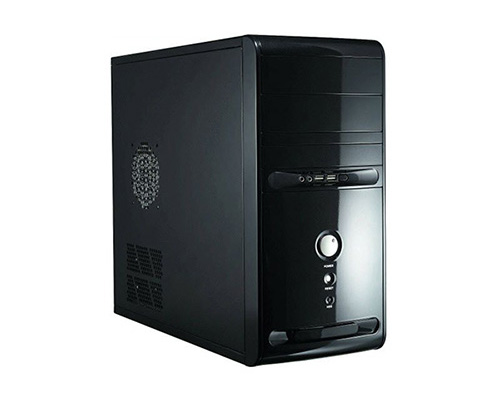
\includegraphics[width=\linewidth]{System-Unit.jpg}
  \caption{PC, steuert den Segway über WLAN}\label{fig:pc}
\endminipage\hfill
\minipage{0.36\textwidth}
  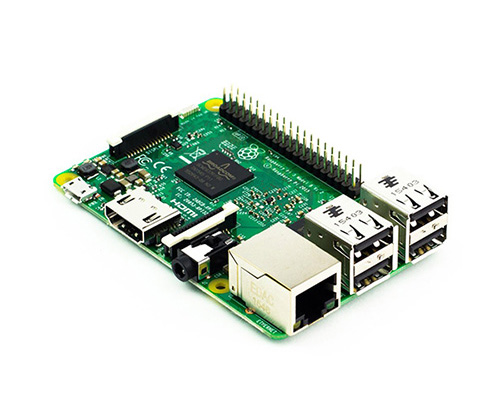
\includegraphics[width=\linewidth]{RaspberryPi3.jpg}
  \caption{Raspberry Pi, kommuniziert mit der Hardware}\label{fig:rpi}
\endminipage\hfill~ \\

~ \hfill
\minipage{0.36\textwidth}
  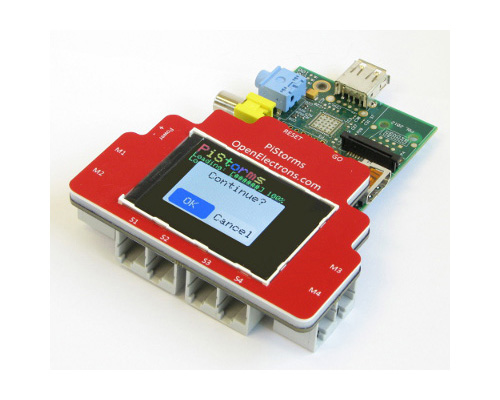
\includegraphics[width=\linewidth]{PiStorms.jpg}
  \caption{PiStorms, koppelt an Lego Komponenten}\label{fig:storms}
\endminipage\hfill
\minipage{0.36\textwidth}
  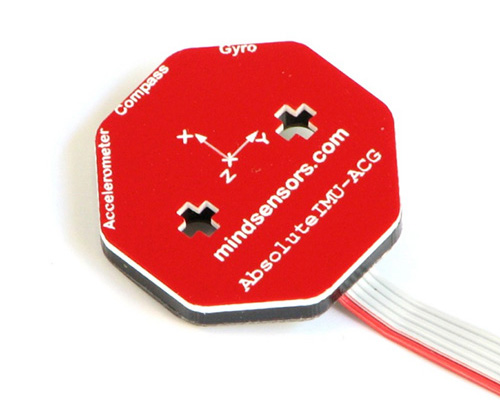
\includegraphics[width=\linewidth]{gyro.jpg}
  \caption{Gyroskop, bestimmt den Neigungswinkel}\label{fig:gyro}
\endminipage\hfill~
\end{figure}

\newpage

Um eine optimale Hardwarezusammensetzung zu erreichen, die möglichst gut mit dem PC über WLAN kommunizieren kann sowie mit wenig Einschränkungen programmierbar ist, soll die EV3-Steuerkomponente durch einen Raspberry Pi (Abbildung \ref{fig:rpi}) ersetzt werden. Dieser wird der mithilfe des PiStorms Base Kits (Abbildung \ref{fig:storms}) mit den Lego Komponenten gekoppelt. Zudem wird der Lego Mindstorms-eigene Gyrosensor durch das Gyroskop von Mindsensors ersetzt, welches genauere Messwerte liefert. 




\subsection*{Aufgabenverteilung}
\begin{itemize}
\item \textbf{Dao Thuy Ngan Tran} - Entwicklung der Steuerungssoftware für den PC, Empfang und Verarbeitung der Sensordaten, Berechnung und Senden der Steuersignale
\item \textbf{Nikita Basargin} - Entwicklung der Hardwarezusammenstellung, Kommunikation mit den Sensoren und Motoren, Empfang und Verarbeitung der Steuersignale
\end{itemize}

\subsection*{Wahl der Vorlesung}
Die Vorlesung Mensch-Maschine-Kommunikation 1 deckt die Grundlagen der Human-Machine Interaction, sowie die grundlegende Funktionsweise verschiedener Sensoren ab. Der Themenbereich der Sensoren lässt sich in den hier beschriebenen Lego Segway integrieren, da dieser durch die Sensordaten mit dem PC kommuniziert.


\end{document}
